%% ---------------------------------------------------------------------------
%% intro.tex
%%
%% Introduction
%%
%% $Id: intro.tex 1477 2010-07-28 21:34:43Z palvarado $
%% ---------------------------------------------------------------------------

\chapter{Entorno del proyecto}
\label{chp:entorno}

La pandemia reciente de COVID-19 ejemplificó el papel de los servicios de video conferencia y de streaming en vivo en la sociedad actual.
Los avances actuales en la velocidad de redes y en la tecnología digital han permitido que estos servicios sean comunes en contextos profesionales, académicos y recreativos.
Por lo tanto, ha aumentado el interés en asegurar una alta calidad de experiencia (QoE, por sus siglas en inglés) para estos servicios.

Uno de los problemas principales que afecta el QoE de los servicios de video conferencia y streaming en vivo son los artefactos de video, como se menciona en \cite{Vranjes2018, Korhonen2018}.
En \cite{Greengrass2009}, los artefactos de video, o simplemente artefactos, se definen como distorsiones en las imágenes desplegadas al usuario con respecto a las imágenes originales capturadas.
Según \cite{Vranjes2018}, los artefactos son causados principalmente por errores o pérdida de datos en la transmisión del video a través de la red, o por pérdidas causadas durante la compresión del video. En la Figura \ref{fig:1.1} se comparan dos versiones de una misma imagen. La Figura \ref{fig:1.1.a} no contiene artefactos de video y la Figura \ref{fig:1.1.b} contiene artefactos de video por pérdida de paquetes.

\begin{figure} [!h]
  \centering
  
  \begin{subfigure}[t]{0.49\textwidth}
    \centering
    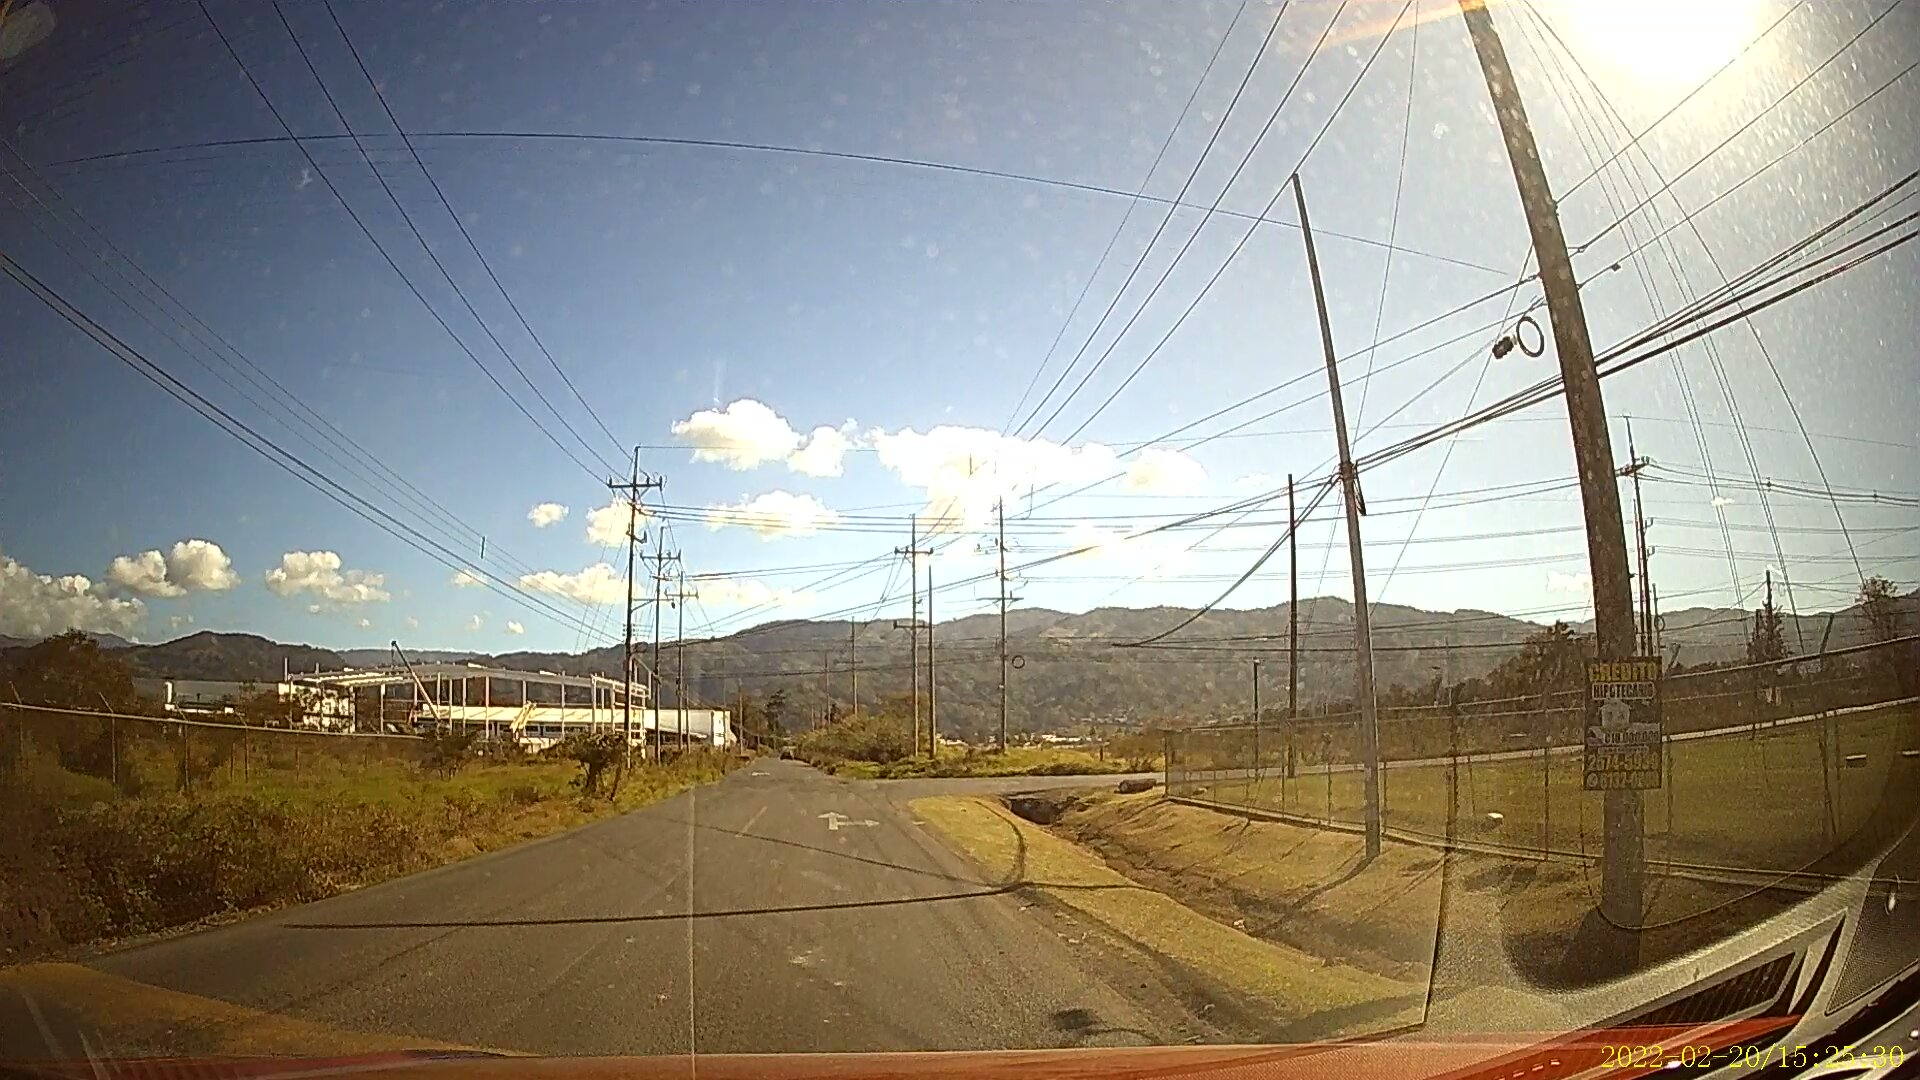
\includegraphics[width=\textwidth]{imgs_27}
    \caption{Cuadro sin pérdida de paquetes}
    \label{fig:1.1.a}
  \end{subfigure}
  \hfill
  \begin{subfigure}[t]{0.49\textwidth}
    \centering
    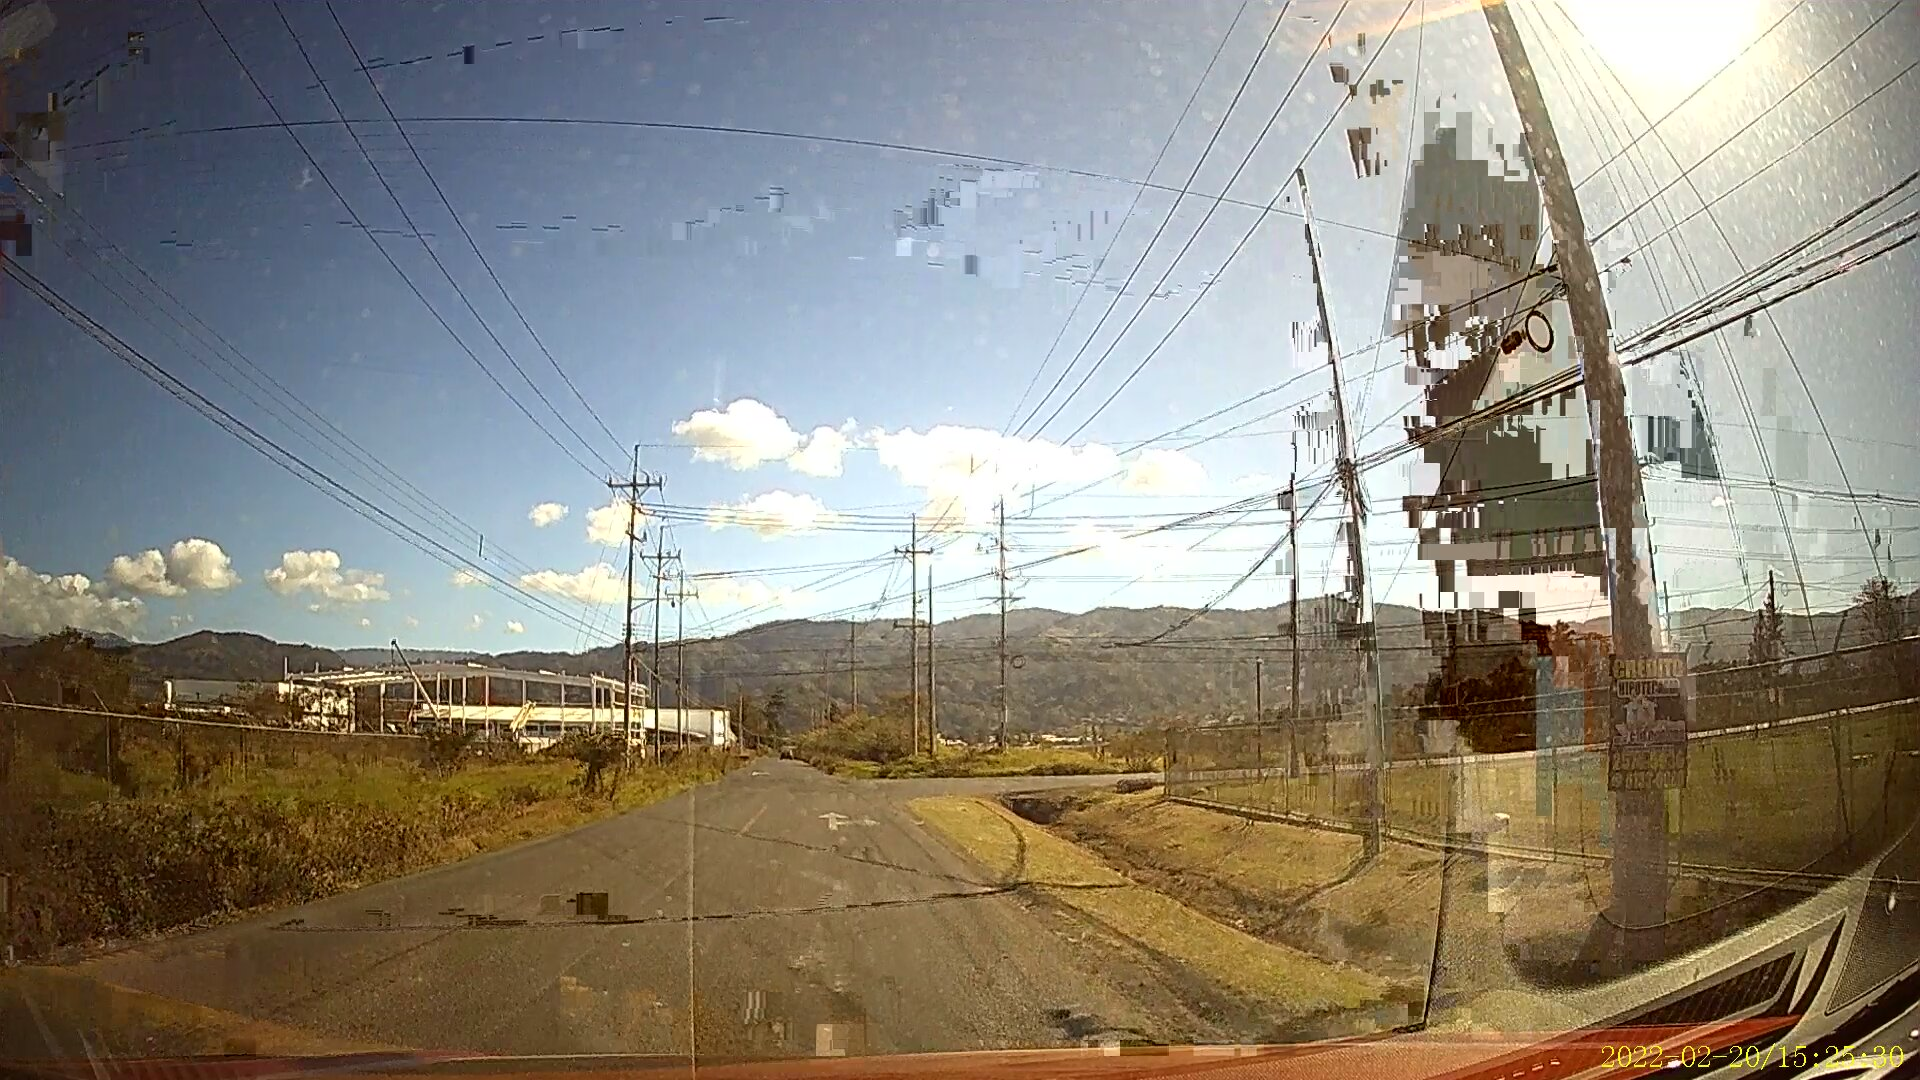
\includegraphics[width=\textwidth]{imgs_with_loss_27}
    \caption{Cuadro con artefactos causados por pérdida de paquetes}
    \label{fig:1.1.b}
  \end{subfigure}
  
  \caption{Ejemplo de artefactos causados por pérdida de paquetes}
  \label{fig:1.1}

\end{figure}

Existen métodos para solucionar los errores de transmisión en la capa de transporte o hasta en la capa de sintaxis de video, como se menciona en \cite{Sanyal2021}.
En estos casos se cuenta con información de cómo están codificados los paquetes de video, por lo cual se simplifica la tarea de detección y corrección de errores.
Cuando el usuario solo cuenta con la información decodificada y descomprimida, es necesario usar métodos para detección y corrección de artefactos que solo cuentan con la información pura de video, como los de \cite{Vranjes2018, Sanyal2021,Goodall2019}.
A estos métodos se le denominan ``métodos sin referencia''.

Los artefactos de video resultan en pérdidas de información del video original. En aplicaciones de video conferencia y streaming en vivo no es posible recuperar la información perdida sin afectar el QoE del usuario.
Para lograr corregir los artefactos de video, los métodos sin referencia deben inferir la información perdida.
Al proceso de restaurar zonas desconocidas de una imagen se le llama ``restauración de video'' \cite{Li2022, Zhou2021}.
La restauración de video, o simplemente restauración, se utiliza comunmente para eliminar la presencia de objetos en un video o una imagen, pero se pueden utilizar para reconstruir zonas de una imagen afectadas por artefactos de video, como se hace en \cite{Dong2023, Brenes2022}.

Los algoritmos modernos de restauración utilizan modelos de aprendizaje de máquina.
Los restauradores de \cite{Li2022, Zhou2021, Liu2021} utilizan ``transformers''.
Los transformers son modelos de aprendizaje de máquina con resultados extraordinarios para tareas de reconstrucción de señales, pero son caros tanto en tiempo como en capacidad de procesamiento \cite{Liu2021}.
Para lograr optimizar el desempeño de estos modelos, se requiere del uso de aceleradores de hardware, el más común siendo el GPU.

Modelos de restauración como el de \cite{Li2022} requiren de máscaras binarias para identificar las zonas que se desea reconstruir.
Por esta razón, se debe detectar la ubicación de los artefactos de video y generar máscaras binarias para luego ser utilizadas en la etapa de reconstrucción de la imagen.

Existen clasificaciones de los distintos tipos de artefactos por pérdida de paquetes \cite{Greengrass2009, Glavota2016}. Estos estudios describen las propiedades estadísticas de los artefactos de video. Por ejemplo, ciertos artefactos de video tienden a tener bordes verticales y horizontales de alto contraste que pueden ser detectados por filtros pasa-altos. En los estándares de compresión de video MPEG y H.26x, los pixeles de una imagen se agrupan en ``macrobloques'', cuales son de grupos de $16 \times 16$ pixeles en la imagen. Pérdidas de paquetes que contienen información de macrobloques resultan en artefactos con bordes bien definidos \cite{Vranjes2019, Glavota2018}.

Los métodos para la detección de artefactos de video de \cite{Vranjes2018, Glavota2018} se centran en algoritmos de filtrado que no involucran aprendizaje de máquina. Estos métodos pueden llegar a procesar más de 30 cuadros de video por segundo contando con solo recursos de CPU, pero sobresimplifican las características de los artefactos de video y no logran alcanzar altas tasas de detección. También existen métodos de detección de artefactos que utilizan redes neuronales, como los de \cite{Goodall2019, Rajasekar2020}. Estos métodos generalizan mejor que los algoritmos de filtrado, pero son más pesados en recursos y requieren de aceleradores, como los GPU, para alcanzar velocidades comparables a los algoritmos de filtrado.

Durante el 2022, el SIPLab desarrolló el proyecto dispTEC2-2022 en conjunto con la empresa RidgeRun para la restauración de video con artefactos por pérdida de paquetes. El proyecto se desarrolló sobre la Jetson TX2 de Nvidia. Este sistema cuenta con un GPU de 256 núcleos CUDA, 4 CPU ARM y 2 CPU Denver. En \cite{Brenes2022} se detalla el desarrollo de la etapa de reconstrucción de imágenes de dispTEC2-2022. Este modelo utiliza el GPU por completo. El modelo de reconstrucción de Brenes requiere de máscaras binarias para ubicar los artefactos en las imágenes de entrada y el proyecto en general carece aún de un método de detección de artefactos.
